% Options for packages loaded elsewhere
% Options for packages loaded elsewhere
\PassOptionsToPackage{unicode}{hyperref}
\PassOptionsToPackage{hyphens}{url}
%
\documentclass[
  english,
  russian,
  12pt,
  a4paper,
  DIV=11,
  numbers=noendperiod]{scrreprt}
\usepackage{xcolor}
\usepackage{amsmath,amssymb}
\setcounter{secnumdepth}{5}
\usepackage{iftex}
\ifPDFTeX
  \usepackage[T1]{fontenc}
  \usepackage[utf8]{inputenc}
  \usepackage{textcomp} % provide euro and other symbols
\else % if luatex or xetex
  \usepackage{unicode-math} % this also loads fontspec
  \defaultfontfeatures{Scale=MatchLowercase}
  \defaultfontfeatures[\rmfamily]{Ligatures=TeX,Scale=1}
\fi
\usepackage{lmodern}
\ifPDFTeX\else
  % xetex/luatex font selection
\fi
% Use upquote if available, for straight quotes in verbatim environments
\IfFileExists{upquote.sty}{\usepackage{upquote}}{}
\IfFileExists{microtype.sty}{% use microtype if available
  \usepackage[]{microtype}
  \UseMicrotypeSet[protrusion]{basicmath} % disable protrusion for tt fonts
}{}
\usepackage{setspace}
% Make \paragraph and \subparagraph free-standing
\makeatletter
\ifx\paragraph\undefined\else
  \let\oldparagraph\paragraph
  \renewcommand{\paragraph}{
    \@ifstar
      \xxxParagraphStar
      \xxxParagraphNoStar
  }
  \newcommand{\xxxParagraphStar}[1]{\oldparagraph*{#1}\mbox{}}
  \newcommand{\xxxParagraphNoStar}[1]{\oldparagraph{#1}\mbox{}}
\fi
\ifx\subparagraph\undefined\else
  \let\oldsubparagraph\subparagraph
  \renewcommand{\subparagraph}{
    \@ifstar
      \xxxSubParagraphStar
      \xxxSubParagraphNoStar
  }
  \newcommand{\xxxSubParagraphStar}[1]{\oldsubparagraph*{#1}\mbox{}}
  \newcommand{\xxxSubParagraphNoStar}[1]{\oldsubparagraph{#1}\mbox{}}
\fi
\makeatother

\usepackage{color}
\usepackage{fancyvrb}
\newcommand{\VerbBar}{|}
\newcommand{\VERB}{\Verb[commandchars=\\\{\}]}
\DefineVerbatimEnvironment{Highlighting}{Verbatim}{commandchars=\\\{\}}
% Add ',fontsize=\small' for more characters per line
\usepackage{framed}
\definecolor{shadecolor}{RGB}{241,243,245}
\newenvironment{Shaded}{\begin{snugshade}}{\end{snugshade}}
\newcommand{\AlertTok}[1]{\textcolor[rgb]{0.68,0.00,0.00}{#1}}
\newcommand{\AnnotationTok}[1]{\textcolor[rgb]{0.37,0.37,0.37}{#1}}
\newcommand{\AttributeTok}[1]{\textcolor[rgb]{0.40,0.45,0.13}{#1}}
\newcommand{\BaseNTok}[1]{\textcolor[rgb]{0.68,0.00,0.00}{#1}}
\newcommand{\BuiltInTok}[1]{\textcolor[rgb]{0.00,0.23,0.31}{#1}}
\newcommand{\CharTok}[1]{\textcolor[rgb]{0.13,0.47,0.30}{#1}}
\newcommand{\CommentTok}[1]{\textcolor[rgb]{0.37,0.37,0.37}{#1}}
\newcommand{\CommentVarTok}[1]{\textcolor[rgb]{0.37,0.37,0.37}{\textit{#1}}}
\newcommand{\ConstantTok}[1]{\textcolor[rgb]{0.56,0.35,0.01}{#1}}
\newcommand{\ControlFlowTok}[1]{\textcolor[rgb]{0.00,0.23,0.31}{\textbf{#1}}}
\newcommand{\DataTypeTok}[1]{\textcolor[rgb]{0.68,0.00,0.00}{#1}}
\newcommand{\DecValTok}[1]{\textcolor[rgb]{0.68,0.00,0.00}{#1}}
\newcommand{\DocumentationTok}[1]{\textcolor[rgb]{0.37,0.37,0.37}{\textit{#1}}}
\newcommand{\ErrorTok}[1]{\textcolor[rgb]{0.68,0.00,0.00}{#1}}
\newcommand{\ExtensionTok}[1]{\textcolor[rgb]{0.00,0.23,0.31}{#1}}
\newcommand{\FloatTok}[1]{\textcolor[rgb]{0.68,0.00,0.00}{#1}}
\newcommand{\FunctionTok}[1]{\textcolor[rgb]{0.28,0.35,0.67}{#1}}
\newcommand{\ImportTok}[1]{\textcolor[rgb]{0.00,0.46,0.62}{#1}}
\newcommand{\InformationTok}[1]{\textcolor[rgb]{0.37,0.37,0.37}{#1}}
\newcommand{\KeywordTok}[1]{\textcolor[rgb]{0.00,0.23,0.31}{\textbf{#1}}}
\newcommand{\NormalTok}[1]{\textcolor[rgb]{0.00,0.23,0.31}{#1}}
\newcommand{\OperatorTok}[1]{\textcolor[rgb]{0.37,0.37,0.37}{#1}}
\newcommand{\OtherTok}[1]{\textcolor[rgb]{0.00,0.23,0.31}{#1}}
\newcommand{\PreprocessorTok}[1]{\textcolor[rgb]{0.68,0.00,0.00}{#1}}
\newcommand{\RegionMarkerTok}[1]{\textcolor[rgb]{0.00,0.23,0.31}{#1}}
\newcommand{\SpecialCharTok}[1]{\textcolor[rgb]{0.37,0.37,0.37}{#1}}
\newcommand{\SpecialStringTok}[1]{\textcolor[rgb]{0.13,0.47,0.30}{#1}}
\newcommand{\StringTok}[1]{\textcolor[rgb]{0.13,0.47,0.30}{#1}}
\newcommand{\VariableTok}[1]{\textcolor[rgb]{0.07,0.07,0.07}{#1}}
\newcommand{\VerbatimStringTok}[1]{\textcolor[rgb]{0.13,0.47,0.30}{#1}}
\newcommand{\WarningTok}[1]{\textcolor[rgb]{0.37,0.37,0.37}{\textit{#1}}}

\usepackage{longtable,booktabs,array}
\usepackage{calc} % for calculating minipage widths
% Correct order of tables after \paragraph or \subparagraph
\usepackage{etoolbox}
\makeatletter
\patchcmd\longtable{\par}{\if@noskipsec\mbox{}\fi\par}{}{}
\makeatother
% Allow footnotes in longtable head/foot
\IfFileExists{footnotehyper.sty}{\usepackage{footnotehyper}}{\usepackage{footnote}}
\makesavenoteenv{longtable}
\usepackage{graphicx}
\makeatletter
\newsavebox\pandoc@box
\newcommand*\pandocbounded[1]{% scales image to fit in text height/width
  \sbox\pandoc@box{#1}%
  \Gscale@div\@tempa{\textheight}{\dimexpr\ht\pandoc@box+\dp\pandoc@box\relax}%
  \Gscale@div\@tempb{\linewidth}{\wd\pandoc@box}%
  \ifdim\@tempb\p@<\@tempa\p@\let\@tempa\@tempb\fi% select the smaller of both
  \ifdim\@tempa\p@<\p@\scalebox{\@tempa}{\usebox\pandoc@box}%
  \else\usebox{\pandoc@box}%
  \fi%
}
% Set default figure placement to htbp
\def\fps@figure{htbp}
\makeatother



\ifLuaTeX
\usepackage[bidi=basic,provide=*]{babel}
\else
\usepackage[bidi=default,provide=*]{babel}
\fi
% get rid of language-specific shorthands (see #6817):
\let\LanguageShortHands\languageshorthands
\def\languageshorthands#1{}


\setlength{\emergencystretch}{3em} % prevent overfull lines

\providecommand{\tightlist}{%
  \setlength{\itemsep}{0pt}\setlength{\parskip}{0pt}}



 
\usepackage[backend=biber,langhook=extras,autolang=other*]{biblatex}
\addbibresource{bib/cite.bib}

\usepackage[]{csquotes}

\usepackage{indentfirst}
\usepackage{float}
\floatplacement{figure}{H}
\IfFileExists{plex-otf.sty}{
  %% Full TeXlive
  \usepackage[math,RM={Scale=0.94},SS={Scale=0.94},SScon={Scale=0.94},TT={Scale=MatchLowercase,FakeStretch=0.9},DefaultFeatures={Ligatures=Common}]{plex-otf}
}{
  %% TinyTeX
  \usepackage{libertine}
}
\KOMAoption{captions}{tableheading}
\makeatletter
\@ifpackageloaded{caption}{}{\usepackage{caption}}
\AtBeginDocument{%
\ifdefined\contentsname
  \renewcommand*\contentsname{Содержание}
\else
  \newcommand\contentsname{Содержание}
\fi
\ifdefined\listfigurename
  \renewcommand*\listfigurename{Список иллюстраций}
\else
  \newcommand\listfigurename{Список иллюстраций}
\fi
\ifdefined\listtablename
  \renewcommand*\listtablename{Список таблиц}
\else
  \newcommand\listtablename{Список таблиц}
\fi
\ifdefined\figurename
  \renewcommand*\figurename{Рисунок}
\else
  \newcommand\figurename{Рисунок}
\fi
\ifdefined\tablename
  \renewcommand*\tablename{Таблица}
\else
  \newcommand\tablename{Таблица}
\fi
}
\@ifpackageloaded{float}{}{\usepackage{float}}
\floatstyle{ruled}
\@ifundefined{c@chapter}{\newfloat{codelisting}{h}{lop}}{\newfloat{codelisting}{h}{lop}[chapter]}
\floatname{codelisting}{Список}
\newcommand*\listoflistings{\listof{codelisting}{Листинги}}
\makeatother
\makeatletter
\makeatother
\makeatletter
\@ifpackageloaded{caption}{}{\usepackage{caption}}
\@ifpackageloaded{subcaption}{}{\usepackage{subcaption}}
\makeatother
\usepackage{bookmark}
\IfFileExists{xurl.sty}{\usepackage{xurl}}{} % add URL line breaks if available
\urlstyle{same}
\hypersetup{
  pdftitle={Отчёт по лабораторной работе 3},
  pdfauthor={Дмитрий Моисеев Вячеславович},
  pdflang={ru-RU},
  hidelinks,
  pdfcreator={LaTeX via pandoc}}


\title{Отчёт по лабораторной работе 3}
\usepackage{etoolbox}
\makeatletter
\providecommand{\subtitle}[1]{% add subtitle to \maketitle
  \apptocmd{\@title}{\par {\large #1 \par}}{}{}
}
\makeatother
\subtitle{Язык разметки Markdown}
\author{Дмитрий Моисеев Вячеславович}
\date{}
\begin{document}
\maketitle

\renewcommand*\contentsname{Содержание}
{
\setcounter{tocdepth}{1}
\tableofcontents
}
\listoffigures
\listoftables

\setstretch{1.5}
\chapter{Цель
работы}\label{ux446ux435ux43bux44c-ux440ux430ux431ux43eux442ux44b}

Целью работы является освоение процедуры оформления отчетов с помощью
легковесного языка разметки Markdown.

\chapter{Задание}\label{ux437ux430ux434ux430ux43dux438ux435}

Здесь приводится описание задания в соответствии с рекомендациями
методического пособия и выданным вариантом.

\chapter{Теоретическое
введение}\label{ux442ux435ux43eux440ux435ux442ux438ux447ux435ux441ux43aux43eux435-ux432ux432ux435ux434ux435ux43dux438ux435}

\textbf{Базовые сведения о Markdown}

Чтобы создать заголовок, используйте знак \#, например: \# This is
heading 1 \#\# This is heading 2 \#\#\# This is heading 3 \#\#\#\# This
is heading 4 Чтобы задать для текста полужирное начертание, заключите
его в двойные звездочки: This text is \textbf{bold}. Чтобы задать для
текста курсивное начертание, заключите его в одинарные звездочки: This
text is \emph{italic}. Чтобы задать для текста полужирное и курсивное
начертание, заключите его в тройные звездочки: This is text is both
\textbf{\emph{bold and italic}}. Блоки цитирования создаются с помощью
символа \textgreater:

\begin{displayquote}
The drought had lasted now for ten million years, and the reign of the
terrible ↪ lizards had long since ended. Here on the Equator, in the
continent which would ↪ one day be known as Africa, the battle for
existence had reached a new climax of ↪ ferocity, and the victor was not
yet in sight. In this barren and desiccated ↪ land, only the small or
the swift or the fierce could flourish, or even hope to ↪ survive.
\end{displayquote}

Упорядоченный список можно отформатировать с помощью соответствующих
цифр: ↪ 1. First instruction 1. Sub-instruction 1. Sub-instruction 1.
Second instruction Чтобы вложить один список в другой, добавьте отступ
для элементов дочернего списка: 1. First instruction 1. Second
instruction 1. Third instruction Неупорядоченный (маркированный) список
можно отформатировать с помощью звездочек или тире: * List item 1 * List
item 2 * List item 3 Чтобы вложить один список в другой, добавьте отступ
для элементов дочернего списка: - List item 1 - List item A - List item
B - List item 2 Синтаксис Markdown для встроенной ссылки состоит из
части {[}link text{]}, представляющей текст гиперссылки, и части
(file-name.md) -- URL-адреса или имени файла, на который дается ссылка:
\href{file-name.md}{link text} или \href{http://example.com/}{link text}
Markdown поддерживает как встраивание фрагментов кода в предложение, так
и их размещение между предложениями в виде отдельных огражденных блоков.
Огражденные блоки кода --- это простой способ выделить синтаксис для
фрагментов кода. Общий формат огражденных блоков кода:

\begin{Shaded}
\begin{Highlighting}[]
\NormalTok{your code goes in here}
\end{Highlighting}
\end{Shaded}

\textbf{Оформление формул в Markdown}

Внутритекстовые формулы делаются аналогично формулам LaTeX. Например,
формула sin2 (𝑥) + cos2 (𝑥) = 1 запишется как
\(\sin^2 (x) + \cos^2 (x) = 1\) Выключение формулы: sin2 (𝑥) + cos2 (𝑥)
= 1 (3.1) со ссылкой в тексте «Смотри формулу (\{-eq. ??\}).»
записывается как \[
\sin^2 (x) + \cos^2 (x) = 1
\] \{\#eq:eq1\} Смотри формулу (\texttt{{[}-@eq:eq1{]}}).

\textbf{Оформление изображений в Markdown}

В Markdown вставить изображение в документ можно с помощью
непосредственного указания адреса изображения. Синтаксис данной команды
выглядит следующим образом:

\includegraphics[width=0.5\linewidth,height=\textheight,keepaspectratio]{image/imgtest.png}

Здесь: • в квадратных скобках указывается подпись к изображению; • в
круглых скобках указывается URL-адрес или относительный путь
изображения, а также (необязательно) всплывающая подсказка, заключённая
в двойные или одиночные кавычки. • в фигурных скобках указывается
идентификатор изображения (\#fig:fig1) для ссылки на него по тексту и
размер изображения относительно ширины страницы (width=90\%) Ссылка на
изображение (рис. ??) может быть оформлена следующим образом: (рис.
\autocite*{fig:fig1})

\textbf{Обработка файлов в формате Markdown}

Для компиляции отчетов по лабораторным работам предлагается использовать
следующий Makefile all: \autocite*{quarto} render clean: -rm -rf
\_output cleanall: clean -rm -rf .quarto

\chapter{Техническое
обеспечение}\label{ux442ux435ux445ux43dux438ux447ux435ux441ux43aux43eux435-ux43eux431ux435ux441ux43fux435ux447ux435ux43dux438ux435}

При выполнении лабораторной работы на своей технике необходимо
установить следующее ПО: • Quarto v1.7.34 (https://www.quarto.org,
https://github.com/quarto-dev/quarto-cli/releases/t ag/v1.7.34). • TeX
Live (https://www.tug.org/texlive/) последней версии. Или TinyTeX
(https://www.yihui. org/tinytex/). На компьютерах в дисплейных классах
факультета физико-математических и естественных наук РУДН все
необходимое ПО установлено.

\chapter{Выполнение лабораторной
работы}\label{ux432ux44bux43fux43eux43bux43dux435ux43dux438ux435-ux43bux430ux431ux43eux440ux430ux442ux43eux440ux43dux43eux439-ux440ux430ux431ux43eux442ux44b}

\begin{enumerate}
\def\labelenumi{\arabic{enumi}.}
\tightlist
\item
  Откроем терминал.
  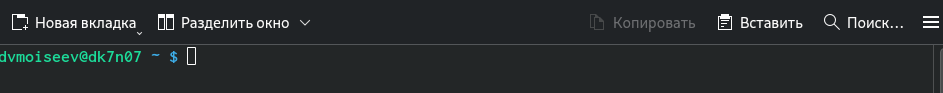
\includegraphics[width=0.5\linewidth,height=\textheight,keepaspectratio]{image/img1.png}
  2.Перейдем в каталог курса, сформированный при выполнении лабораторной
  работы № 2: cd
  \textasciitilde/work/study/2025-2026/\enquote{Архитектура
  компьютера}/arch-pc/
  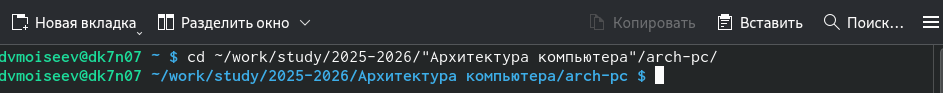
\includegraphics[width=0.5\linewidth,height=\textheight,keepaspectratio]{image/img2.png}
  Обновим локальный репозиторий, скачав изменения из удаленного
  репозитория с помощью команды git pull
  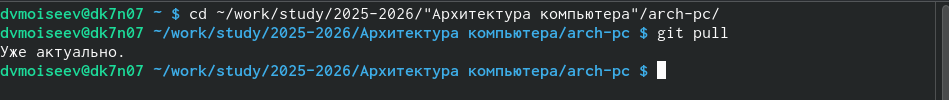
\includegraphics[width=0.5\linewidth,height=\textheight,keepaspectratio]{image/img3.png}
  3.Перейдите в каталог с шаблоном отчета по лабораторной работе № 3: cd
  \textasciitilde/work/study/2025-2026/\enquote{Архитектура
  компьютера}/arch-pc/labs/lab03/report
\end{enumerate}

4.Проведите компиляцию шаблона с использованием Makefile. Для этого
введите команду make
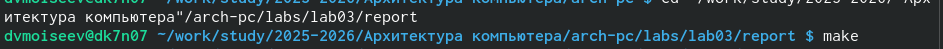
\includegraphics[width=0.5\linewidth,height=\textheight,keepaspectratio]{image/img4.png}
При успешной компиляции должны сгенерироваться файлы report.pdf и
report.docx. Откройте и проверьте корректность полученных файлов.
5.Удалите полученный файлы с использованием Makefile. Для этого введите
команду make clean
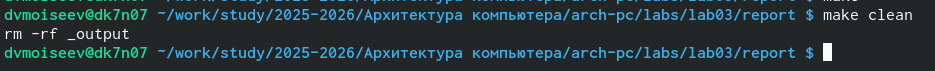
\includegraphics[width=0.5\linewidth,height=\textheight,keepaspectratio]{image/img5.png}
Проверьте, что после этой команды файлы report.pdf и report.docx были
удалены. 6.6. Откройте файл report.md c помощью любого текстового
редактора, например gedit gedit report.md

Внимательно изучите структуру этого файла
\includegraphics[width=0.5\linewidth,height=\textheight,keepaspectratio]{image/img6.png}
7.Заполните отчет и скомпилируйте отчет с использованием Makefile.
Проверьте корректность полученных файлов. (Обратите внимание, для
корректного отображения скриншотов они должны быть размещены в каталоге
image.) 8.Загрузите файлы на Github. cd
\textasciitilde/work/study/2025-2026/\enquote{Архитектура
компьютера}/arch-pc git add . git commit -am \enquote*{feat(main): add
files lab-3} git push
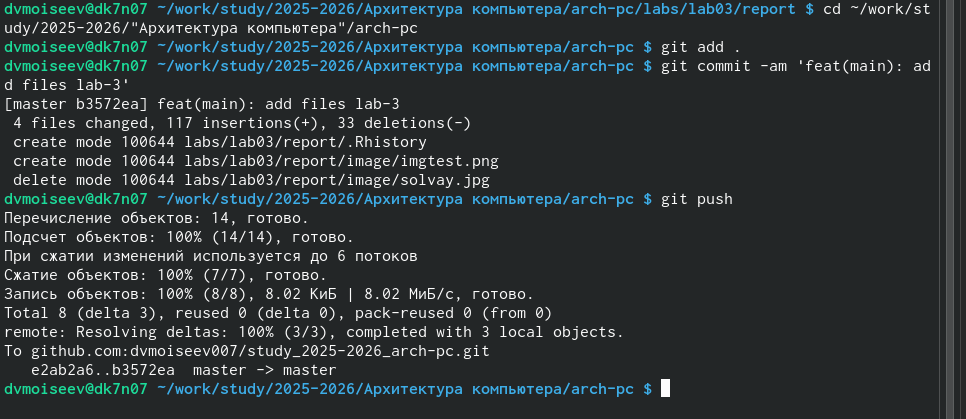
\includegraphics[width=0.5\linewidth,height=\textheight,keepaspectratio]{image/img8.png}
\# Выводы

В рамках данной работы мы освоили процедуры оформления отчетов с помощью
легковесного языка разметки Markdown.

\chapter*{Список
литературы}\label{ux441ux43fux438ux441ux43eux43a-ux43bux438ux442ux435ux440ux430ux442ux443ux440ux44b}
\addcontentsline{toc}{chapter}{Список литературы}

\printbibliography[heading=none]





\end{document}
